\section{Introduction}

The PSBLAS library, developed with the aim to facilitate the
parallelization of computationally intensive scientific applications,
is designed to address parallel implementation of iterative solvers
for sparse linear systems through the distributed memory paradigm.  It
includes routines for multiplying sparse matrices by dense matrices,
solving block diagonal systems with triangular diagonal entries,
preprocessing sparse matrices, and contains additional routines for
dense matrix operations.  The current implementation of PSBLAS
addresses a distributed memory execution model operating with message
passing. However, the overall design does not preclude different
implementation paradigms, such as those based on a shared memory
model.

The PSBLAS library is internally implemented in a mixture of
Fortran~77 and Fortran~95~\cite{metcalf} programming languages. A
similar approach has been advocated by a number of authors,
e.g.~\cite{machiels}.  Moreover, the Fortran~95 facilities for dynamic
memory management and interface overloading greatly enhance the usability of the PSBLAS
subroutines. In this way, the library can take care of runtime memory
requirements that are quite difficult or even impossible to predict at
implementation or compilation time.  The following presentation of the
PSBLAS library follows the general structure of the proposal for
serial Sparse BLAS~\cite{sblas97}, which in its turn is based on the
proposal for BLAS on dense matrices~\cite{BLAS1,BLAS2,BLAS3}.

The applicability of sparse iterative solvers to many different areas
causes some terminology problems because the same concept may be
denoted through different names depending on the application area. The
PSBLAS features presented in this section will be discussed mainly in terms of finite
difference discretizations of Partial Differential Equations (PDEs).
However, the scope of the library is wider than that: for example, it
can be applied to finite element discretizations of PDEs, and even to
different classes of problems such as nonlinear optimization, for
example in optimal control problems.

The design of a solver for sparse linear systems is driven by many
conflicting objectives, such as limiting occupation of storage
resources, exploiting regularities in the input data, exploiting
hardware characteristics of the parallel platform.  To achieve an
optimal communication to computation ratio on distributed memory
machines it is essential to keep the {\em data locality} as high as
possible; this can be done through an appropriate data allocation
strategy.  The choice of the preconditioner is another very important
factor that affects efficiency of the implemented application. Optimal
data distribution requirements for a given preconditioner may conflict
with distribution requirements of the rest of the solver. Finding the
optimal trade-off may be very difficult because it is application
dependent.  Possible solution to these problems and other important
inputs to the development of the PSBLAS software package has come from
an established experience in applying the PSBLAS solvers to
computational fluid dynamics applications.

\section{General overview}
\label{sec:overview} 
The PSBLAS library is designed to handle the implementation of
iterative solvers for sparse linear systems on distributed memory
parallel computers.  The system coefficient matrix $A$ must be square;
it may be real or complex, nonsymmetric, and its sparsity pattern
needs not to be symmetric.  The serial computation parts are based on
the serial sparse BLAS, so that any extension made to the data
structures of the serial kernels is available to the parallel
version. The overall design and parallelization strategy have been
influenced by the structure of the ScaLAPACK parallel
library~\cite{scalapack}.  The layered structure of the PSBLAS library
is shown in figure~\ref{fig:psblas} ; lower layers of the library
indicate an encapsulation relationship with upper layers. The ongoing
discussion focuses on the Fortran~95 layer immediately below the
application layer; two examples of iterative solvers built through the
PSBLAS routines, will be also given in Section~\ref{sec:itmethd}.  The
serial parts of the computation on each process are executed through
calls to the serial sparse BLAS subroutines. In a similar way, the
inter-process message exchanges are implemented through the Basic
Linear Algebra Communication Subroutines (BLACS) library~\cite{BLACS}
that guarantees a portable and efficient communication layer. The
Message Passing Interface code is encapsulated within the BLACS
layer. However, in some cases, MPI routines are directly used either
to improve efficiency or to implement communication patterns for which
the BLACS package doesn't provide any method.

\begin{figure}[h] \begin{center}
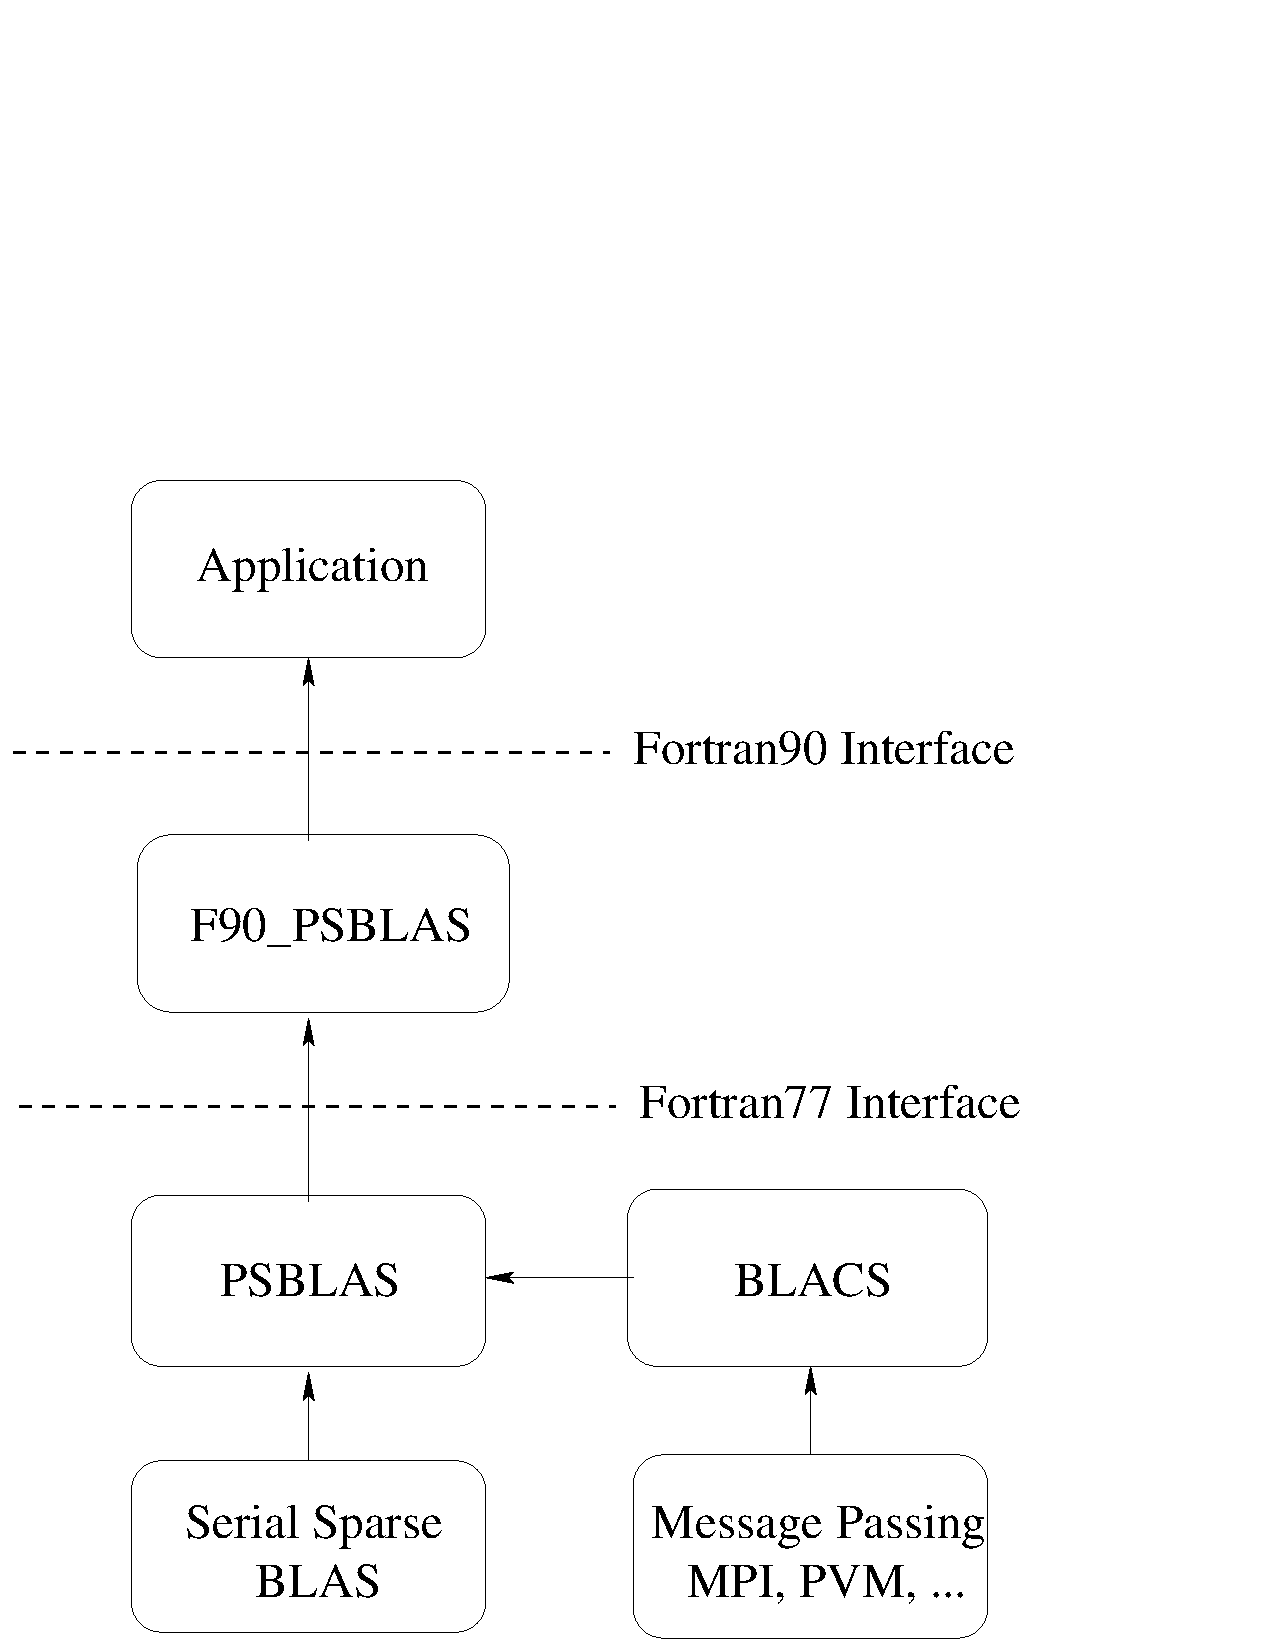
\includegraphics[scale=0.45]{figures/psblas}
\end{center}
\caption{PSBLAS library components hierarchy.\label{fig:psblas}}
\end{figure}

The PSBLAS library consists of two classes of subroutines that is, the
{\em computational routines} and the {\em auxiliary routines}.  The
computational routine set includes:

\begin{itemize}
\item Sparse matrix by dense matrix product; \item Sparse triangular
systems solution for block diagonal matrices;
\item Vector and matrix norms;
\item Dense matrix sums;
\item Dot products.
\end{itemize} 
The auxiliary routine set includes:
\begin{itemize}
\item Communication descriptors allocation;
\item Dense and sparse matrix allocation;
\item Dense and sparse matrix build and update;
\item Sparse matrix and data distribution preprocessing.
\end{itemize} 

The following naming scheme has been adopted for all the symbols
internally defined in the PSBLAS software package:
\begin{itemize}
\item all the symbols (i.e. subroutine names, data types...) are
  prefixed by \verb|psb_| 
\item all the data type names are suffixed by \verb|_type|
\item all the constant values are suffixed by \verb|_|
\item all the subroutine names follow the rule \verb|psb_xxname| where
  \verb|xx| can be either:
  \begin{itemize}
  \item \verb|ds|: the routine is related to dense data, 
  \item \verb|sp|: the routine is related to sparse data, 
  \item \verb|cd|: the routine is related to communication descriptor (see~\ref{sec:datastruct}).
  \end{itemize}
  For example the \verb|psb_dsins|, \verb|psb_spins| and
  \verb|psb_cdins| perform the same action (see~\ref{sec:toolsrout}) on
  dense matrices, sparse matrices and communication descriptors
  respectively.
  Interface overloading allows the usage of the same subroutine
  interfaces for both real and complex data.
\end{itemize}

%%% Local Variables: 
%%% mode: latex
%%% TeX-master: "userguide"
%%% End: 
